
%(BEGIN_QUESTION)
% Copyright 2007, Tony R. Kuphaldt, released under the Creative Commons Attribution License (v 1.0)
% This means you may do almost anything with this work of mine, so long as you give me proper credit

Identify which of these valve bodies is {\it direct-acting} and which is {\it reverse-acting}:

$$\includegraphics[width=15.5cm]{i01629x01.eps}$$

Similarly, identify which of these valve actuators is {\it direct-acting} and which is {\it reverse-acting}:

$$\includegraphics[width=15.5cm]{i01629x02.eps}$$

Finally, identify {\it two combinations} of valve bodies and actuators that will make an {\it air-to-close} valve.

\underbar{file i01629}
%(END_QUESTION)





%(BEGIN_ANSWER)

I recommend 2 points for correctly identifying the valve types, 2 points for correctly identifying the actuator types, and 3 points for each correct valve/actuator combination (10 points total).

$$\includegraphics[width=15.5cm]{i01629x03.eps}$$

$$\includegraphics[width=15.5cm]{i01629x04.eps}$$

For an air-to-close valve, combine a {\it direct-acting valve and direct-acting actuator}, or combine a {\it reverse-acting valve and reverse-acting actuator}.

%(END_ANSWER)





%(BEGIN_NOTES)

{\bf This question is intended for exams only and not worksheets!}.

%(END_NOTES)


